\documentclass[dvipdfmx,12pt]{beamer}

\usepackage{bxdpx-beamer}
\usepackage{pxjahyper}
\usepackage{minijs}
\usetheme{AnnArbor}
\usepackage{mathpazo}
\usepackage{amsmath,amssymb}
\usepackage{graphicx}
\usepackage{array}
\usepackage{tikz}
\usepackage{wrapfig}
\usepackage{float}
\usepackage{here}
\usepackage{lscape}
\setbeamertemplate{navigation symbols}{}

\title{Reference Dependence and Monetary Incentive}
\subtitle{-Evidence from Major League Baseball-}
\author{Reio TANJI}
\date{Dec 14th, 2018}
\institute{Osaka University}

\begin{document}

\begin{frame}\frametitle{}
\titlepage
\end{frame}

\section{Introduction}
\begin{frame}\frametitle{Abstract}
  \begin{itemize}
    \item Empirical research that specifies the existance of reference point dependence observed in field setting:

    We pick up evidence of Major League Baseball (MLB)

    \item Players take some round numbers of the batting performance indexes as reference points, and adjust their effort level to meet the goals

    \item There are NOT observed any evidence for the monetary incentives that is paid to the players if they achieve these internal goals
  \end{itemize}
\end{frame}

\begin{frame}\frametitle{Introduction}
  \begin{itemize}
    \item Reference dependence is one of the two main charactaristics of the Tversky and Kahneman (1992)'s prospect theory:

    Individuals evaluate outcomes by the relative value to their internal benchmarks, or reference point, not by their absolute ones.

    \item Prospect theory enabled us to interpret some inconsistent empirical decision making with the traditional microeconomic theory, by applying additional assumptions.

    \item There are a lot of following researches that tests the reference dependence in field or laboratory settings.
  \end{itemize}
\end{frame}

\section*{Table of Contents}
\begin{frame}\frametitle{Contents}
  \tableofcontents
\end{frame}

\section{literature and Contribution}
\begin{frame}\frametitle{Literature}
  Pope and Simonsohn (2011)
  \begin{itemize}
    \item presents three empirical evidences that verify the reference dependence, with the reference points ``round numbers.''

    \item One of them picked up Major League Baseball (MLB) players, about the observed attitude to their performance indexes.

    \item MLB position players manipulate their batting-average (AVG), in order to meet their internal goals: .300

    \item As a results, there is observed excess mass, or ``bunching'' around .300 of AVG.
  \end{itemize}
\end{frame}

\begin{frame}\frametitle{Contribution}
\begin{itemize}
  \item Professional athletes receive monetary rewards according to the contracts they signed.

  \item Their contracts might include some incentivesed parts, which pay them additional bonus when their AVG reaches a certain cutoff point.

  \item If so, the observed behavior might be caused by the discontinuity of their profit function, not by the reference dependence.

  \item The contribution of our research is to examine this: examine if there exists any monetary incentives that make players make effort to the cutoff point.
\end{itemize}
\end{frame}

\section{Frameworks and Empirical Methods}
\begin{frame}\frametitle{Theoretical Frameworks}
  \begin{tabular}{lrr}
    \begin{minipage}[H]{0.4\textwidth}
      \begin{figure}[H]
        \begin{tikzpicture}[domain = 0:4, samples = 200, >= stealth]
          \draw[->](-0.5, 0) -- (4.2, 0) node[right]{$x$};
          \draw[->](0, -0.5) -- (0, 3.7) node[above]{$u(x)$};
          \draw[-](2.2, -0.1) -- (2.2, 0.1);
          \draw[domain=0:2.2,samples=200,>=stealth] plot (\x, {sqrt(\x)});
          \draw[domain=2.2:4.1,samples=200,>=stealth] plot (\x, {sqrt(\x) + 0.8});
          \draw (0, 0) node[below left]{O};
          \draw (2.2, -0.3) node {$r$};
        \end{tikzpicture}
        \scriptsize
        \caption{discontinuous utility function}
        \label{jump}
      \end{figure}
      \end{minipage} &
      \begin{minipage}[H]{0.5\textwidth}
        \small
        \begin{itemize}
          \item Following Allen et al. (2016) assume utility function $u(x)$ that jumps at the cutoff point, or the reference point.

          $x$ stands for the performance index.

          \item This disconituity generates excess mass, or ``bunching'' around the possible reference point.

          \item We consider if this utility is derived by the descontinuous design of the monetary reward of the players.

        \end{itemize}
      \end{minipage}
  \end{tabular}

\end{frame}

\begin{frame}\frametitle{Specification: Manipulation}
  \begin{itemize}
    \item We exploit the McCrary (2007)'s manipulation test, which is used in regression discontinuity design.

    \item Local-linear regression of undersmoothed histgram around the given cutoff point: .300 of AVG, 20 homeruns, \ldots

    \item
  \end{itemize}
\end{frame}

\begin{frame}\frametitle{Specification: Contract Design}
  \begin{itemize}
    \item Discontinuity of the contract design is tested by RDD methodology:

    \[
    w_{it} = \beta_0 X_{it} + \beta_1 \text{ABOVE}_{it}
    \]

    \item To check the robustness of our results, we also conduct the same local regression including the interaction term of $X_{it}$ and $\text{ABOVE}_{it}$.

    \[
    w_{it} = \beta_0 X_{it} + \beta_1 \text{ABOVE}_{it} + \beta_2 X_{it} \times \text{ABOVE}_{it}
    \]

  \end{itemize}
\end{frame}

\begin{frame}\frametitle{Data}
  We obtain information about the players' stats (indexes) and annual salary.
  \begin{itemize}
    \item Stats Data
    \begin{itemize}
      \item From \textit{fangraphs}

      \item Play stats from 1957 to 2018

      \item We restrict the sample to the players with at least 200 plate-appearances $N=18143$
    \end{itemize}
    \item Salary Data
    \begin{itemize}
      \item From \textit{USA TODAY} and \textit{Baseball Prospectus}

      \item Salary information from 1987 to 2017 $N=8915$
    \end{itemize}
  \end{itemize}
\end{frame}

\section{Results}
\begin{frame}\frametitle{Results: Manipulation}
  \begin{figure}
    \centering
    \caption{Histgram of Batting-Average}        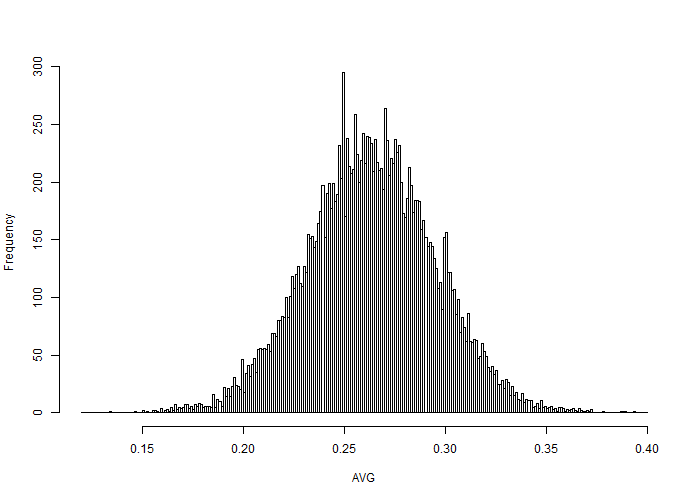
\includegraphics[keepaspectratio, scale = 0.35, angle=0]{graphs/hist_AVG_all.png}
    \label{AVG_Histgram}
  \end{figure}

\end{frame}

\begin{frame}
  \begin{figure}
    \centering
    \caption{Discontinuity at .300 of AVG}
    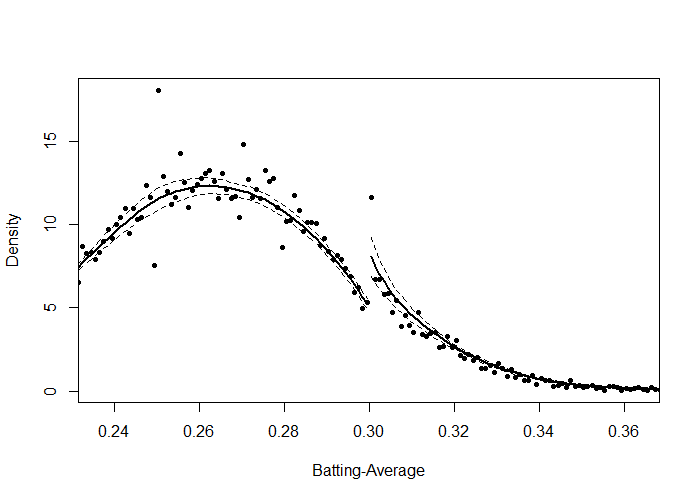
\includegraphics[keepaspectratio, scale = 0.5, angle = 0]{graphs/AVG_300.png}
    \label{DCdensity_AVG_300}

  \end{figure}
\end{frame}

\begin{frame}
  \begin{table}
    \tiny
    \centering
    \caption{Test for Manipulation, leastPA $= 200$}
    \begin{tabular}{lcccccc}\hline
      index & type & cutpoint & binsize & bandwidth & $\theta$ & $z$
      \\ \hline \hline
      AVG & rate & .300 & .001 & .019 &  .499 & 7.442*** \\
      & & & & & (.067) & \\
      & & .250 & .001 & .024 & .212 & 5.061*** \\
      & & & & & (.042) & \\
      OBP & rate & .350 & .001 & .024 &  .139 & 2.854** \\
      & & & & & (.049) &  \\
      HR & cumulative & 20 & 1 & 5.309 & .259 & 3.465*** \\
      & & & & & (.075)  & \\
      RBI & cumulative & 100 & 4 & 15.423 & .311 & 3.295*** \\
      & & & & & (.094) & \\
      SB & cumulative & 30 & 1 & 10.000 & .529 & 4.274*** \\
      & & & & & (.124) & \\
      & & 40 & 1 & 11.505 & .481 & 2.764** \\
      & & & & & (.174) & \\
      PA & cumulative & 500 & 1 & .003 & .160 & 2.515* \\
      & & & & &(.063) & \\
      H & cumulative & 200 & 1 & 18.922 & .453 & 2.547 * \\
      & & & & & (.178) & \\ \hline \hline
      Note & \multicolumn{6}{r}{
      ***: $p<0.1\%$, **: $p<1\%$, *: $p<5\%$.
      }\\
      \multicolumn{7}{r}{
      Bandwidth is optimized following the method of McCrary(2008).
      }
    \end{tabular}
    \label{Bunch-True}
  \end{table}
\end{frame}

\begin{frame}\frametitle{}

\end{frame}

\begin{frame}\frametitle{Results: Contract Design}
  \begin{table}[!]
    \caption{RDD Test for Monetary Incentives}
    \label{RDD_A}
    \tiny
    \centering
    \begin{tabular}{lccccccc}\hline
      index,cutpoint & Other Control & bw type & bandwidth
      & Observations & Estimate & Std. Error & $z$
      \\ \hline \hline
      AVG, .300 & No &LATE & .084 & 8514 & .047 & .061 & .773 \\
      & &Half-BW &  .042 & 5599 & .088 & .075 & 1.174 \\
      & & Double-BW & .170 & 8915  & .067 & .056 & 1.184 \\ \cline{3-8}

      & Yes &LATE & .045 & 5930 & .034 & .056 & .615 \\
      & &Half-BW &  .023 & 3005 & .061 & .077 & .788 \\
      & & Double-BW & .090 & 8605  & .016 & .045 & .354 \\ \hline

      AVG, .250 & No &LATE & .036 & 6110 & .019 & .068 & .286 \\
      & &Half-BW &  .018 & 3496 & .015 & .092 & .161 \\
      & & Double-BW & .072 & 8539  & .034 & .054 & .636 \\ \cline{3-8}

      & Yes &LATE & .048 & 7271 & .070 & .052 & 1.340 \\
      & &Half-BW &  .024 & 4402 & .066 & .069 & .953 \\
      & & Double-BW & .096 & 8810  & .075 & .044 & 1.713 \\ \hline

      HR, 20 & No & LATE & 3.32 & 1315 & .071 & .175 & .406 \\
      & & Half-BW & 1.66 & 562 & .073 & .127 & .576 \\
      & & Double-BW & 6.64 & 2582 & -.004 & .109 & -.034 \\ \cline{3-8}

      & Yes & LATE & 3.30 & 1307 & -.002 & .141 & -.015\\
      & & Half-BW &1.65 & 560 & .030 & .102 & .299 \\
      & & Double-BW & 6.61 & 2558 & -.032 & .088 & -.364 \\ \hline

      OBP, .350 & No &LATE & .044 & 6440 & -.038 & .065 & -.592 \\
      & & Half-BW & .021 & 3542 & -.076 & .089 & -.849 \\
      & & Double-BW & .087 & 8656 & -.029 & .051 & -.570 \\ \cline{3-8}

      & Yes & LATE & .045 & 6525 & -.013 & .049 & -.272 \\
      & & Half-BW & .022 & 3673 & -.055 & .069 & -.807 \\
      & &Double-BW & .089 & 8637 & .004 & .039 & .107 \\ \hline

      RBI, 100 & No & LATE & 4.08 & 393 & .072 & .289 & .250 \\
      & &Half-BW & 2.04 & 228 & .282 & .400 & .707 \\
      & &Double-BW & 8.16 & 714 & .008 & .185 & .043 \\ \cline{3-8}

      & Yes & LATE & 4.04 & 390 & .018 & .209 & .086 \\
      & & Half-BW & 2.02 & 227 & -.042 & .324 & .130 \\
      & & Double-BW & 8.07 & 708 & .056 & .127 & .435 \\ \hline

      H, 200& No & LATE & 3.173 & 75 & -.786 & .396 & -1.985* \\
      & & Half-BW & 1.587 & 35 & .386 & .271 & -1.421 \\
      & & Double-BW & 6.347 & 137 & -.061 & .309 & -.199 \\ \cline{3-8}

      & Yes & LATE & 3.175 & 75 & -.420 & 1.042 & -.403 \\
      & & Half-BW & 1.587 & 35 & -4.779 & .576 & -8.288** \\
      & & Double-BW & 6.349 & 137 & -.109 & .413 & -.265 \\ \hline

      SB, 30 & No & LATE & 3.39 & 282 & .962 & .372 & 2.585** \\
      & &Half-BW & 1.70 & 134 & .920 & .263 & 3.492*** \\
      & &Double-BW & 8.16 & 714 & .008 & .185 & 2.941** \\ \cline{3-8}

      & Yes & LATE & 3.40 & 282 & .379 & .297 & 1.271 \\
      & & Half-BW & 1.70 & 134 & .290 & .249 & 1.163 \\
      & & Double-BW & 6.79 & 533 & .408 & .180 & 2.260* \\ \hline

      SB, 40 & No & LATE & 3.16 & 134 & -1.276 & .453 & -2.818** \\
      & &Half-BW & 1.58 & 56 & -.736 & .383 & -1.924 \\
      & &Double-BW & 6.32 & 245 & -.712 & .313 & -2.274* \\ \cline{3-8}

      & Yes & LATE & 3.16 & 134 & -.346 & .396 & -.875 \\
      & & Half-BW & 1.58 & 56 & -.313 & .429 & -.730 \\
      & & Double-BW & 6.33 & 245 & -.115 & .244 & -.472 \\ \hline

      Note: & \multicolumn{7}{r}{***: $p<0.1\%$, **: $p<1\%$, *: $p<5\%$.} \\
      & \multicolumn{7}{r}{Bandwidth is optimized following the method of Imbens-Kalyanaraman.}
    \end{tabular}
  \end{table}
\end{frame}

\begin{frame}\frametitle{}

\end{frame}

\begin{frame}\frametitle{Summary}

\end{frame}

\begin{frame}\frametitle{Discussion}
  \begin{itemize}
    \item By-Time analysis
    \begin{itemize}
      \item Replicate the same examination, but now we devide the sample by histrical terms:
      \begin{itemize}
        \item Before the system of free agency regulated (-1975)

        \item Before the Strike of Players Association (-1994)

        \item Before \textit{Moneyball} (Lewis) was published (-2003)

        \item Afterward (2004-)
      \end{itemize}
    \end{itemize}
  \end{itemize}

\end{frame}

\section{Conclusions}
\begin{frame}\frametitle{Conclusion}
  Main Findings
  \begin{enumerate}
    \item Players manipulate their performance indexes to meet them with some round numbers.

    \item There exist no monetary incentives in their contracts that makes players to do so.

    \item Tendency of the manipulation changes through the history of baseball.

    - Among them, especially, .300 of AVG shows consistent results, which shows it is solid benchmarks for the players.
  \end{enumerate}
\end{frame}

\begin{frame}\frametitle{Reference}
  \tiny
  \begin{thebibliography}{99}
    \bibitem PPope and Simonsohn. 2011.
    Round Numbers as Goals: Evidence From Baseball, SAT Takers, and the Lab
    \textit{Psychological Science} 22(1) 7179

    \bibitem HHakes and Sauer. 2006.
    An Economic Evaluation of the Moneyball Hypothesis
    \textit{Journal of Economic Perspectives} Volume 20, Number 3―Summer 2006―Pages 173185

    \bibitem AAllen, Dechow, Pope and Wu. 2016.
    Reference-Dependent Preferences: Evidence from Marathon Runners \textit{Management Science} 63(6):1657-1672.

    \bibitem PPope and Schweizer. 2011.
    Is Tiger Woods Loss Averse? Persistent Bias in the Face of Experience, Competition, and High Stakes
    \textit{American Economic Review} 101 (February 2011): 129157

    \bibitem{}Kahneman and Tversky. 1979.
    Prospect Theory: An Analysis of Decision under Risk.
    \textit{Econometrica}
    Journal of the Econometric Society47 (2):263291.

    \bibitem{}McCrary. 2007.
    Manipulation of the running variable in the regression discontinuity design: A density test
    \textit{Journal of Econometrics} 142 (2008) 698–714

    \bibitem{}Krautmann and Oppenheimer. 2002.
    Contract Length and the Return to Performance in Major League Baseball
    \textit{Journal of Sports Economics} February 2002

    \bibitem{}Tversky and Kahneman. 1992.
    Advances in Prospect Theory: Cumulative Representation of Uncertainty
    \textit{Journal of Risk and Uncertainty}, 5:297-323 (1992)

    \bibitem{}Imbens and Kalyanaraman. 2009.
    \textit{NBER Working Paper Series.} 14726

    \bibitem{}Alex Rees-Jones. 2018.
    Quantifying Loss-Averse Tax Manipulation
    \textit{Review of Economic Studies} (2018) 85, 1251–1278
  \end{thebibliography}

\end{frame}

\section*{Appendix}
\begin{frame}

\end{frame}

\end{document}
